\documentclass{beamer}

\usepackage[ruled]{algorithm2e}
\SetKw{KwRet}{return}
\SetKwRepeat{Repeat}{repeat}{until}
\usepackage{amsmath}
\usepackage{mathtools}

\usetheme{AnnArbor}
\usecolortheme{crane}
\usefonttheme[onlymath]{serif}

\title{Deep Learning - Foundations and Concepts}
\subtitle{Chapter 15. Discrete Latent Variables}
\author{nonlineark@github}
\date{\today}

\begin{document}

\begin{frame}
    \titlepage
\end{frame}

\begin{frame}
    \frametitle{Outline}
    \tableofcontents
\end{frame}

\section{\texorpdfstring{$K$}{K}-means Clustering}

\begin{frame}
    \frametitle{$K$-means clustering}
    \begin{block}{Problem}
        Suppose we have a data set $\{x^{1},\hdots,x^{N}\}$ consisting of $N$ observations of a $D$-dimensional Euclidean variable $x$. Partition the data set into some number $K$ of clusters, where we will suppose for the moment that the value of $K$ is given.
    \end{block}
\end{frame}

\begin{frame}
    \frametitle{$K$-means clustering}
    \begin{block}{Problem'}
        Find:
        \begin{itemize}
            \item $K$ cluster centers: $\mu_{1},\hdots,\mu_{K}\in\mathbb{R}^{D}$.
            \item $N$ data point assignment: $r^{1},\hdots,r^{N}\in\{\mathrm{e}_{1},\hdots,\mathrm{e}_{K}\}$.
        \end{itemize}
        such that the error function:
        \begin{equation*}
            J=\sum_{n=1}^{N}\sum_{k=1}^{K}r^{n}_{k}||x^{n}-\mu_{k}||^{2}
        \end{equation*}
        which represents the sum of the squares of the distances of each data point to its assigned cluster center, is minimized.
    \end{block}
\end{frame}

\begin{frame}
    \frametitle{$K$-means clustering}
    We can do this through an iterative procedure:
    \begin{enumerate}
        \item Choose some initial values for the $\{\mu_{k}\}$.
        \item E step: Minimize $J$ with respect to the $\{r^{n}_{k}\}$, keeping the $\{\mu_{k}\}$ fixed.
        \item M step: Minimize $J$ with respect to the $\{\mu_{k}\}$, keeping the $\{r^{n}_{k}\}$ fixed.
        \item Go to step 2 until convergence.
    \end{enumerate}
\end{frame}

\begin{frame}
    \frametitle{$K$-means clustering}
    Consider the E step. It's easy to see that we should assign the $n$th data point to the closest cluster center:
    \begin{equation*}
        r^{n}_{k}=\begin{cases}
            1,\qquad\textrm{if }k=\arg\min_{j}||x^{n}-\mu_{j}||^{2} \\
            0,\qquad\textrm{otherwise}
        \end{cases}
    \end{equation*}
    For the M step:
    \begin{align*}
        \frac{\partial{}J}{\partial{}\mu_{k}}&=2\sum_{n=1}^{N}r^{n}_{k}(x^{n}-\mu_{k})^{T} \\
        \mu_{k}&=\frac{\sum_{n=1}^{N}r^{n}_{k}x^{n}}{\sum_{n=1}^{N}r^{n}_{k}}
    \end{align*}
    so $\mu_{k}$ is equal to the mean of all the data points $x_{n}$ assigned to cluster $k$.
\end{frame}

\begin{frame}
    \frametitle{$K$-means clustering}
    \begin{algorithm}[H]
        \caption{$K$-means algorithm}
        $\{r^{n}_{k}\}\gets{}0$\;
        \Repeat{$\{r^{n}_{k}\}=\{\prescript{\mathrm{old}}{}{r}^{n}_{k}\}$}{
            $\{\prescript{\mathrm{old}}{}{r}^{n}_{k}\}\gets\{r^{n}_{k}\}$\;
            \For{$n\gets{}1$ \KwTo $N$}{
                $k\gets\arg\min_{j}||x^{n}-\mu_{j}||^{2}$\;
                $r^{n}_{k}\gets{}1$\;
                $r^{n}_{j\ne{}k}\gets{}0$\;
            }
            \For{$k\gets{}1$ \KwTo $K$}{
                $\mu_{k}\gets\frac{\sum_{n=1}^{N}r^{n}_{k}x^{n}}{\sum_{n=1}^{N}r^{n}_{k}}$\;
            }
        }
        \Return{$\{\mu_{k}\},\{r^{n}_{k}\}$}\;
    \end{algorithm}
\end{frame}

\begin{frame}
    \frametitle{$K$-means clustering}
    When updating the prototype vectors, we can also derive a sequential update in which, for each data point $x^{n}$ in turn, we update the nearest prototype $\mu_{k}$ using:
    \begin{equation*}
        \prescript{\textrm{new}}{}{\mu}_{k}=\prescript{\textrm{old}}{}{\mu}_{k}+\frac{1}{N_{k}}(x^{n}-\prescript{\textrm{old}}{}{\mu}_{k})
    \end{equation*}
    where $N_{k}$ is the number of data points that have so far been used to update $\mu_{k}$.
\end{frame}

\begin{frame}
    \frametitle{Image segmentation}
    Using the $K$-means algorithm to perform (toy) image segmentation:
    \begin{itemize}
        \item Each pixel in an image is a point in a three-dimensional space comprising the intensities of the red, blue and green channels.
        \item We treat each pixel in the image as a separate data point.
        \item We can apply the $K$-means algorithm to these pixels, and redraw the image in which we replace each pixel by the center $\mu_{k}$ to which that pixel has been assigned.
    \end{itemize}
\end{frame}

\begin{frame}
    \frametitle{Image segmentation}
    \begin{figure}
        \caption{Application of the $K$-means clustering algorithm to image segmentation}
        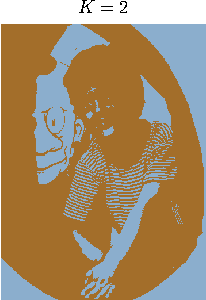
\includegraphics[width=0.2\textwidth]{Figure_3_a.pdf}
        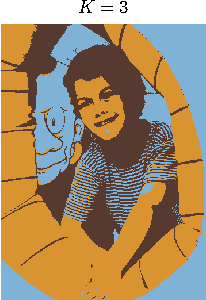
\includegraphics[width=0.2\textwidth]{Figure_3_b.pdf}
        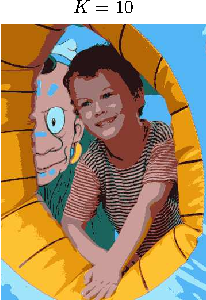
\includegraphics[width=0.2\textwidth]{Figure_3_c.pdf}
        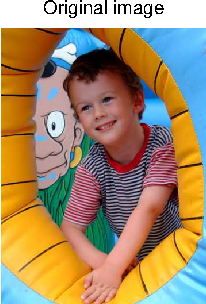
\includegraphics[width=0.2\textwidth]{Figure_3_d.pdf}
    \end{figure}
\end{frame}

\begin{frame}
    \frametitle{Image segmentation}
    Using the $K$-means algorithm to perform lossy data compression:
    \begin{itemize}
        \item For each of the $N$ data points, we store only the identity $k$ of the cluster to which it is assigned.
        \item We also store the values of the $K$ cluster centers $\{\mu_{k}\}$.
    \end{itemize}
    This framework is often called vector quantization, and the vectors $\{\mu_{k}\}$ are called codebook vectors.
\end{frame}

\section{Mixtures of Gaussians}

\begin{frame}
    \frametitle{Mixtures of Gaussians}
    Formulation of Gaussian mixtures in terms of discrete latent variables:
    \begin{itemize}
        \item Let $z$ be a $K$-dimensional binary random variable having a $1$-of-$K$ representation:
        \begin{itemize}
            \item $p(z)=\prod_{k=1}^{K}\pi_{k}^{z_{k}}$, where $0\le\pi_{k}\le{}1$ and $\sum_{k=1}^{K}\pi_{k}=1$.
        \end{itemize}
        \item Let $x$ be a random variable whose distribution given a particular value for $z$ is a Gaussian:
        \begin{itemize}
            \item $p(x|z)=\prod_{k=1}^{K}\mathcal{N}(x;\mu_{k},\Sigma_{k})^{z_{k}}$.
        \end{itemize}
    \end{itemize}
\end{frame}

\begin{frame}
    \frametitle{Mixtures of Gaussians}
    We see that the marginal distribution for $x$ is given by:
    \begin{equation*}
        p(x)=\sum_{z}p(z)p(x|z)=\sum_{k=1}^{K}\pi_{k}\mathcal{N}(x;\mu_{k},\Sigma_{k})
    \end{equation*}
    which is a Gaussian mixture. We are now able to work with the joint distribution $p(x,z)$ instead of the marginal distribution $p(x)$, and this will lead to significant simplifications.
\end{frame}

\begin{frame}
    \frametitle{Mixtures of Gaussians}
    Let's calculate $\gamma(z_{k})=p(z_{k}=1|x)$:
    \begin{equation*}
        p(z_{k}=1|x)=\frac{p(z_{k}=1)p(x|z_{k}=1)}{\sum_{k'=1}^{K}p(z_{k'}=1)p(x|z_{k'}=1)}=\frac{\pi_{k}\mathcal{N}(x;\mu_{k},\Sigma_{k})}{\sum_{k'=1}^{K}\pi_{k'}\mathcal{N}(x;\mu_{k'},\Sigma_{k'})}
    \end{equation*}
    We will view $\pi_{k}$ as the prior probability of $z_{k}=1$, and the quantity $\gamma(z_{k})$ as the corresponding posterior probability once we have observed $x$. $\gamma(z_{k})$ can also be viewed as the responsibility that component $k$ takes for explaining the observation $x$.
\end{frame}

\begin{frame}
    \frametitle{Likelihood function}
    Suppose we have a data set of observations $\{x^{1},\hdots,x^{N}\}$, and we wish to model this data using a mixture of Gaussians. The log of the likelihood function is given by:
    \begin{equation*}
        L=\sum_{n=1}^{N}\log(\sum_{k=1}^{K}\pi_{k}\mathcal{N}(x^{n};\mu_{k},\Sigma_{k}))
    \end{equation*}
\end{frame}

\begin{frame}
    \frametitle{Likelihood function}
    We see that:
    \begin{itemize}
        \item Due to the presence of the summation over $k$ that appears inside the logarithm, when maximizing this log likelihood function, we will no longer obtain a closed-form solution.
        \item The maximization of the log likelihood function is not a well-posed problem, because singularities will occur whenever one of the Gaussian components collapses onto a specific data point.
        \item Identifiability issue: For any given (non-degenerate) point in the space of parameter values, there will be a further $K!-1$ additional points all of which give rise to exactly the same distribution.
    \end{itemize}
\end{frame}

\begin{frame}
    \frametitle{Maximum likelihood}
    Let's find the conditions that must be satisfied at a maximum of the log likelihood function:
    \begin{align*}
        0&=\frac{\partial{}L}{\partial\mu_{k}}=\sum_{n=1}^{N}\gamma(z^{n}_{k})(x^{n}-\mu_{k})^{T}\Sigma_{k}^{-1}\implies\mu_{k}=\frac{1}{N_{k}}\sum_{n=1}^{N}\gamma(z^{n}_{k})x^{n} \\
        0&=\frac{\partial{}L}{\partial\Lambda_{k}}(H)=\frac{1}{2}\sum_{n=1}^{N}\gamma(z^{n}_{k})\mathrm{tr}((\Sigma_{k}-(x^{n}-\mu_{k})(x^{n}-\mu_{k})^{T})H) \\
        &\implies\Sigma_{k}=\frac{1}{N_{k}}\sum_{n=1}^{N}\gamma(z^{n}_{k})(x^{n}-\mu_{k})(x^{n}-\mu_{k})^{T} \\
        \lambda&=\frac{\partial{}L}{\partial\pi_{k}}=\frac{N_{k}}{\pi_{k}}\implies\pi_{k}=\frac{N_{k}}{N}
    \end{align*}
    where $N_{k}=\sum_{n=1}^{N}\gamma(z^{n}_{k})$. We can interpret $N_{k}$ as the effective number of points assigned to cluster $k$.
\end{frame}

\begin{frame}
    \frametitle{Maximum likelihood}
    We can maximize the log likelihood function through an iterative procedure:
    \begin{enumerate}
        \item Choose some initial values for the means, covariances and mixing coefficients.
        \item E step: Use the current values for the parameters to evaluate the posterior probabilities.
        \item M step: Use these probabilities to re-estimate the means, covariances and mixing coefficients.
        \item Go to step 2 until convergence.
    \end{enumerate}
\end{frame}

\begin{frame}
    \frametitle{Maximum likelihood}
    \scalebox{0.8}{
        \begin{algorithm}[H]
            \caption{EM algorithm for a Gaussian mixture model}
            \Repeat{convergence}{
                \For{$n\gets{}1$ \KwTo $N$}{
                    \For{$k\gets{}1$ \KwTo $K$}{
                        $\gamma(z^{n}_{k})=\frac{\pi_{k}\mathcal{N}(x^{n};\mu_{k},\Sigma_{k})}{\sum_{k'=1}^{K}\pi_{k'}\mathcal{N}(x^{n};\mu_{k'},\Sigma_{k'})}$\;
                    }
                }
                \For{$k\gets{}1$ \KwTo $K$}{
                    $N_{k}\gets\sum_{n=1}^{N}\gamma(z^{n}_{k})$\;
                    $\mu_{k}\gets\frac{1}{N_{k}}\sum_{n=1}^{N}\gamma(z^{n}_{k})x^{n}$\;
                    $\Sigma_{k}\gets\frac{1}{N_{k}}\sum_{n=1}^{N}\gamma(z^{n}_{k})(x^{n}-\mu_{k})(x^{n}-\mu_{k})^{T}$\;
                    $\pi_{k}\gets\frac{N_{k}}{N}$\;
                }
                $L\gets\sum_{n=1}^{N}\log(\sum_{k=1}^{K}\pi_{k}\mathcal{N}(x^{n};\mu_{k},\Sigma_{k}))$\;
            }
            \Return{$\{\mu_{k}\},\{\Sigma_{k}\},\{\pi_{k}\}$}\;
        \end{algorithm}
    }
\end{frame}

\end{document}